%
% teil3.tex -- Beispiel-File für Teil 3
%
% (c) 2020 Prof Dr Andreas Müller, Hochschule Rapperswil
%
% !TEX root = ../../buch.tex
% !TEX encoding = UTF-8
%
\section{Rechenzeitoptimierung
\label{wavelets:section:teil3}}
\rhead{Rechenzeitoptimierung}
Ab diesem Zeitpunkt war ein lauffähiger CWT-Code vorhanden, wie die
Abbildung \ref{wavelet:fig:ErsteAnwendung}, zeigt können damit gut
aufgelöste und vor allem korrekte Resultate erzielt werden.
Die Problematik ist aber die Anfangs erwähnte Rechenzeit.
An der Stelle wurde ein grosser Effort in die Minimierung der
Rechenzeit gesteckt.
Im Folgenden werden die wichtigsten Optimierungsansätze angeschaut.

%\subsection{Reduktion der Berechnungspunkte
%\label{wavelets:subsection:ReduktionBerechnungspunkte}}
%Die Verrechnung soll auf die stellen reduziert werden, an denen es auch etwas zu rechnen gibt. Das kann über einen einfach If-Case gemacht werden. Am Phasengang des gleichen Beispiels wie oben kann man die Minimierung %abbilden (Abbildung \ref{wavelet:fig:CwtCalcReduct}).

%\begin{figure}
%	\centering
%	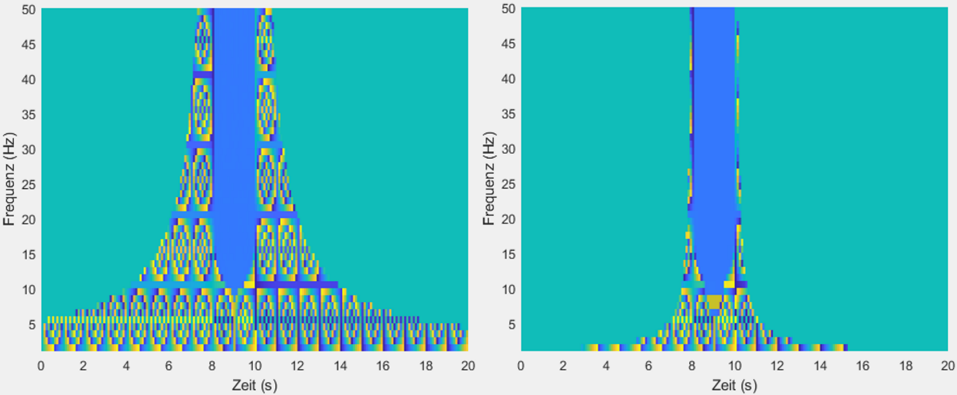
\includegraphics[width=0.5\textwidth]{papers/wavelets/images/13_CWT-CalcReduct.png}
%	\caption{Reduktion der Berechnungen illustriert am Phasengang}
%	\label{wavelet:fig:CwtCalcReduct}
%\end{figure}

\subsection{Elimination der For-Schleifen
	\label{wavelets:subsection:EliminationForSchlaufen}}
Bis an hin wurde die CWT über eine Verschachtelung von For-Schleifen
berechnet.
Die ersten beiden Schleifen, mit der Frequenz $a$ und der Verschiebung
$b$, sind ihrer Rechenzeit überschaubar.
In Kombination mit der letzten Schleife, welche die einzelnen
Auswertungspunkte abfährt, steigt aber der Rechenaufwand mit
zunehmender Abtastrate extrem an.
Die neue Idee war, das Wavelet nicht ständig über diese letzte
For-Schleife an den einzelnen Auswertungspunkten $x(n)$ errechnen
zu müssen, sondern das Signal und das Wavelet als fertige Arrays
mittels Skalarprodukt direkt zu verrechnen.

\begin{figure}
	\centering
	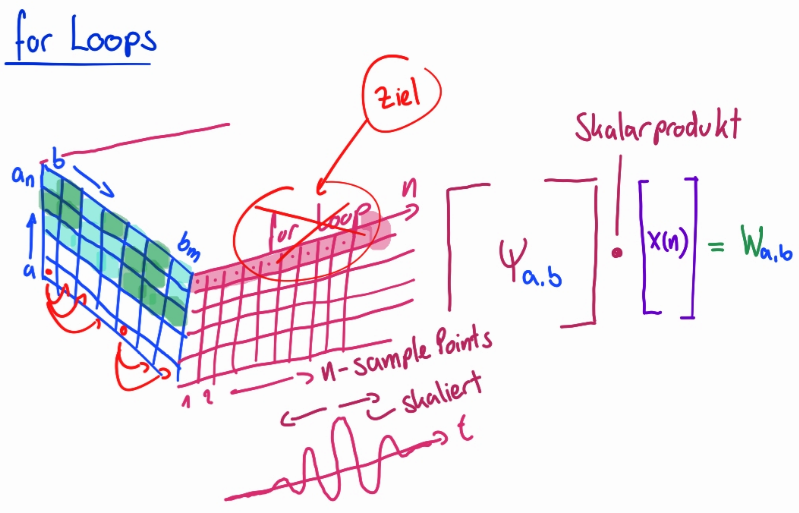
\includegraphics[width=0.65\textwidth]{papers/wavelets/images/14-1_EliminationForLoops.png}
	\caption{Zeitreduktion mittels direkter Skalarprodukt
	Verrechnung der Signal- und Wavelet-Arrays}
	\label{wavelet:fig:EliminationForLoops}
\end{figure}

Die Abbildung \ref{wavelet:fig:EliminationForLoops} soll die Idee
dahinter Erläutern.
Die Frontfläche des Bildes zeigt die beiden Laufvariablen Frequenz
$a$ und Verschiebung $b$.
Anstatt für jede Position $a$, $b$ über eine weitere For-Schleife
die einzelnen Werte zu erzeugen, wird wie in der Summenformel
\[
W_{a,b}
=
\sum_{a=f_0}^{a_n}\sum_{b=0}^{b_m}\frac{1}{N(a)}\sum_{n=0}^{N-1}
x(n)\cdot\psi\left(\frac{n-b}{a}\right)
\]
neu direkt für jede Position $a$, $b$ ein Wavelet-Array erstellt.
Ein solches Array kann in der Abbildung
\ref{wavelet:fig:EliminationForLoops} als ein an der Stelle $a_n$
und $b_m$ in Tiefenrichtung zeigendes Element des Quaders verstanden
werden.
Der Wert der Wavelettransformation wird danach direkt aus dem
Skalarprodukt von einem solchen Arrayelement an der Stelle $a_n$,
$b_m$ sowie dem Signal $x(n)$ generiert.
Die zeitliche Reduktion der Laufzeit von etwa 50\% widerspiegelt
sich auch im Code in Abbildung \ref{wavelet:fig:EliminationForLoopCode}
wieder.

\begin{figure}
	\centering
	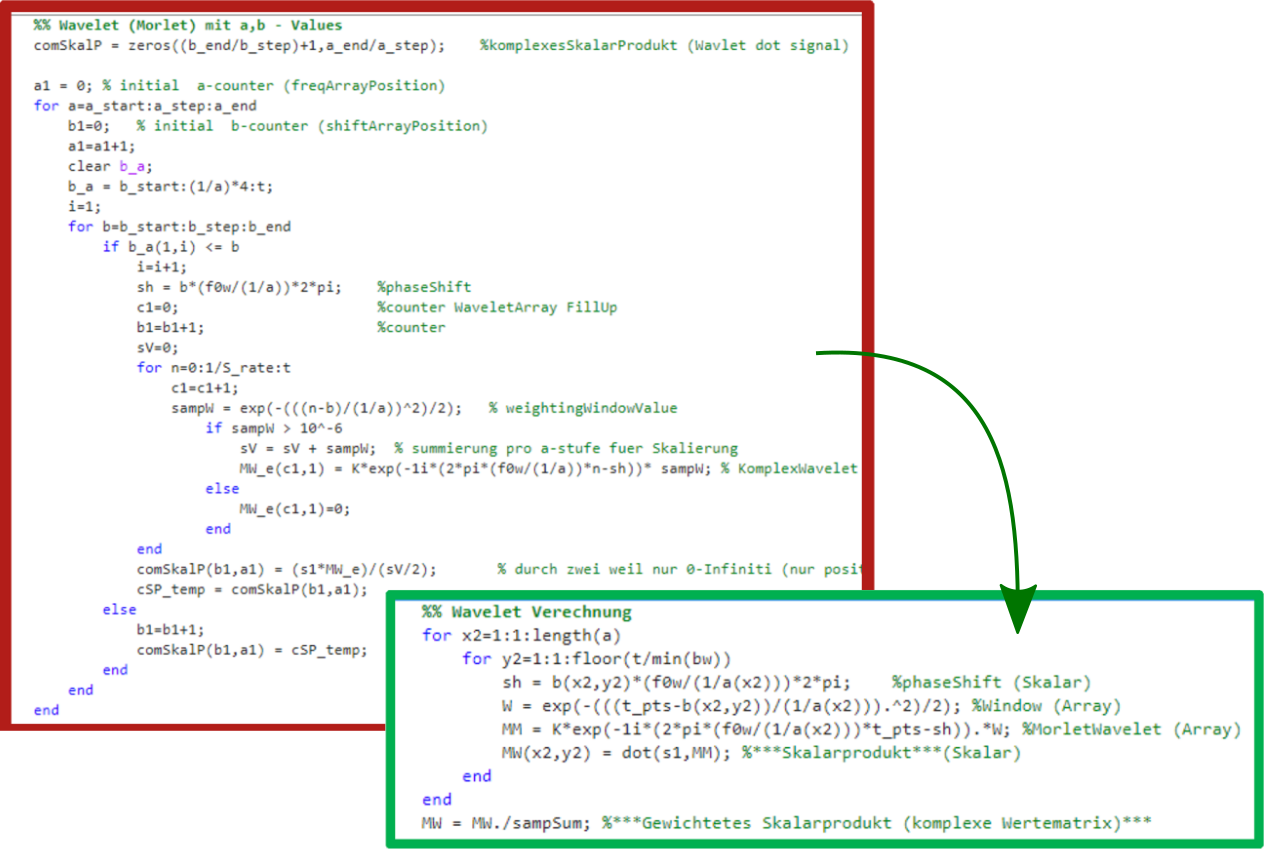
\includegraphics[width=\textwidth]{papers/wavelets/images/14-2_CodeSkalarProd.png}
	\caption{Code Reduktion durch die Implementierung des
	Skalarproduktes zwischen Signal und Wavelet-Array.
	Diese visuelle Reduktion widerspiegelt sich auch in der
	Rechenzeit des CWT-Programm.}
	\label{wavelet:fig:EliminationForLoopCode}
\end{figure}

\subsection{Adaptierter Zeitschritt
	\label{wavelets:subsection:AdaptierterZeitschritt}}
Der letzte Schritt, um das Programm noch schneller zu machen, ist
angelehnt an das Konzept der Filterbank bei der DWT (diskrete
Wavelettransformation).
Dabei soll die zeitliche Auflösung der Periodenbreite des Wavelets
angepasst werden, denn ein tieffrequentes Wavelet besitzt eine
zeitlich viel höhere Ausdehnung als ein hochfrequentes stark
komprimiertes Wavelet (Abbildung \ref{wavelet:fig:adaptedShift_b})
und es ist nicht sinnvoll das Wavelet bei allen Frequenzen um
dieselbe Zeitdauer zu verschieben.

\begin{figure}
	\centering
	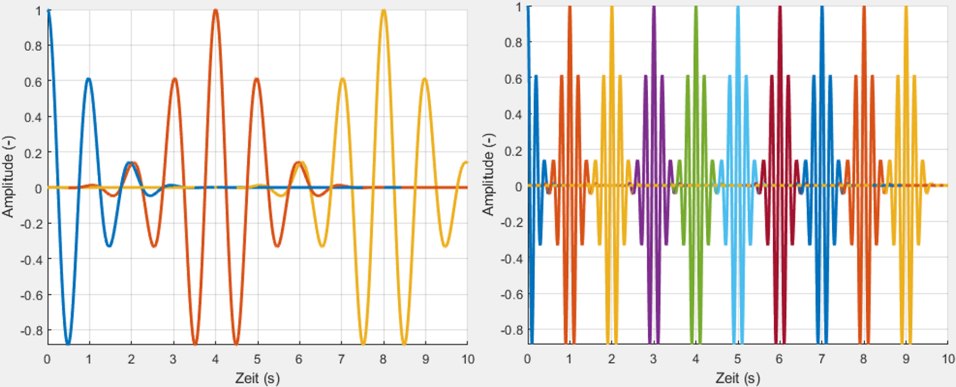
\includegraphics[width=\textwidth]{papers/wavelets/images/15-1_adaptedShift-b.png}
	\caption{Darstellung der zeitlichen Ausdehnung eines Morlet-Wavelets
	bei zwei unterschiedlichen Frequenzen.}
	\label{wavelet:fig:adaptedShift_b}
\end{figure}

Die Frequenzauflösung war schon einstellbar als Vielfaches der
gewählten Grundfrequenz, was in dem Zusammenhang hier noch versucht
wurde, im spezifischen für das Filterbank adaptierte CWT, ist eine
Frequenzerhöhung zu Radix zwei, d.~h.~ die Auswertungsfrequenz des
Wavelets wurde mit $f_\text{wavelet} = 2^k$ pro Stufe $k = 0, 1,
2$ bis $K$ erhöht.
Dadurch wird eine Rasterung der $a$, $b$ Fläche wie im linken Bild
\ref{wavelet:fig:adaptedFrequndTime} erzeugt.

\begin{figure}
	\centering
	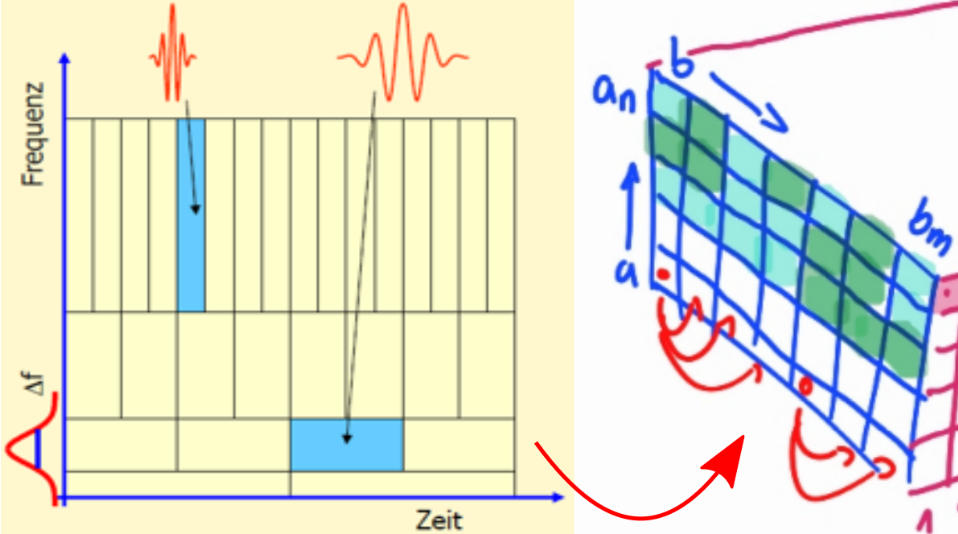
\includegraphics[width=0.75\textwidth]{papers/wavelets/images/15-2_adaptedFrequndTime.png}
	\caption{Variable Verschiebung sowie Skalierung angelehnt an die Idee der Filterbank bei der DWT.
Im Programm umgesetzt an der $a_n \times b_m$ Matrix.}
	\label{wavelet:fig:adaptedFrequndTime}
\end{figure}

Dabei entsteht aber noch eine Schwierigkeit, die es zu lösen gilt.
Die Darstellung ist zwar eindeutig für das Verständnis, entspricht
aber nicht einer $n \times m$ Matrix, mit der man rechnen könnte.
Die Lösung dieses Problems ist andeutungsweise im rechten Bild mit
den roten Pfeilen dargestellt.
Die Anzahl an Spalten ist abhängig von der höchsten Frequenz und
der dafür gewählten zeitlichen Verschiebung.
Für die zeitliche Verschiebung $b$, wurde ein $\Delta t=\frac{1}{a}\cdot2$
gewählt, da das gerade einer 50\% Überlappung entspricht.
Die Anzahl Spalten ergibt sich demnach aus
\begin{equation}
	N_\text{Spalten}=\frac{T_\text{Signal}}{\frac{1}{a_\text{max}}}\cdot2.
	\label{wavelets:equation7}
\end{equation}

%(Abbildung \ref{wavelet:fig:filterbankFillUp})

\begin{figure}
	\centering
	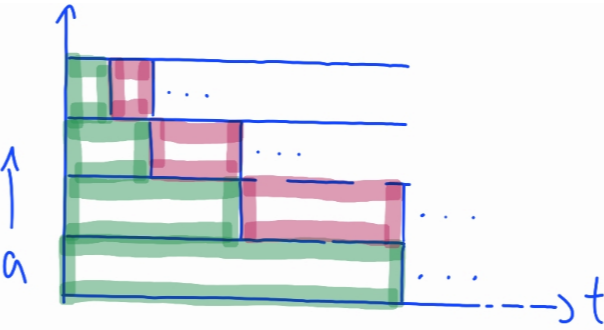
\includegraphics[width=0.35\textwidth]{papers/wavelets/images/16-1_filterbankFillUp_1.png}
	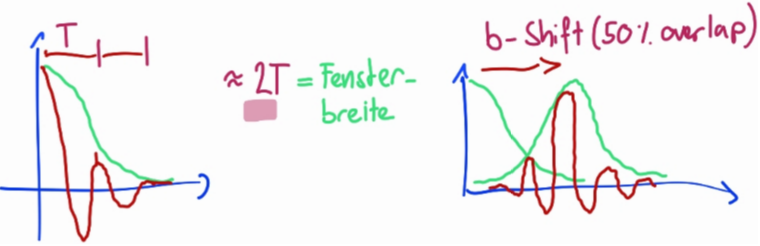
\includegraphics[width=0.6\textwidth]{papers/wavelets/images/16-2_filterbankFillUp_2.png}
	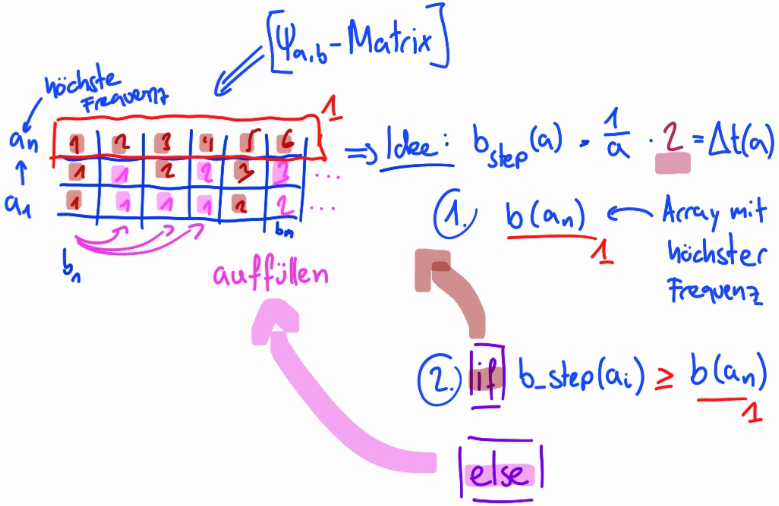
\includegraphics[width=0.6\textwidth]{papers/wavelets/images/16-3_filterbankFillUp_3.png}
	\caption{Schematische Idee hinter der Matrixbefüllung mit
	einer an die Frequenz $a$ angepassten Verschiebung $b(a)$.
	Die Darstellung zur Linken zeigt die Halbierung der
	Periodenlänge des Wavelets und somit die Erhöhung der
	Frequenz $a$ um $2^k$.
	Zur Rechten ist der Faktor 2 für die 50\% Überlappung des
	Wavelets graphisch angegeben.
	Die Überlappung dient in diesem Fall dem Verhindern von
	Informationsverlust und führt zu einer natürlichen Glättung
	in der Visualisierung der Resultate.
	In der unteren Graphik ist ein Pseudo-Code angegeben der
	die Matrixbefüllung im Programm beschreibt.
	Dabei wird für jede Frequenz $a$ ein der Ausdehnung des
	Wavelets entsprechender Zeitschritt errechnet.
	Die Spaltenanzahl wird dabei über die Verschiebungswerte
	von $b(a_\text{max})$ definiert.
	Wavelets mit einer tieferen Frequenz und somit grösserer
	Ausdehnung als das Wavelet mit $a_\text{max}$, besitzen
	dadurch einen Überschuss an Spalten. Die überschüssigen
	Spalten werden nur mit dem ausgehenden Skalarprodukt zwischen
	Wavelet- und Signalarray befüllt und die Berechnung auf an
	die Verschiebung $b(a)$ angepasste Spalten reduziert.}
	\label{wavelet:fig:filterbankFillUp}
\end{figure}

Um diesen Befüllungsprozess zu veranschaulichen, im Folgenden ein
kleines Beispiel für die Frequenzen 1\,Hz – $2^k$\,Hz, wobei $k_{max}
= 3$.
Die Skalierung $a$ wurde übrigens im Code so implementiert, dass
sie direkt der Frequenz entspricht und nicht bloss eine Skalierung
gegenüber der Grundfrequenz $f_0$ beschreibt.

\begin{figure}
	\centering
	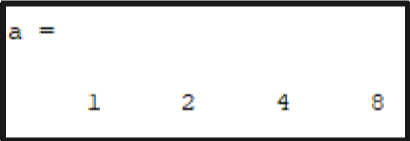
\includegraphics[width=0.2\textwidth]{papers/wavelets/images/17-1_a-Array.png}
	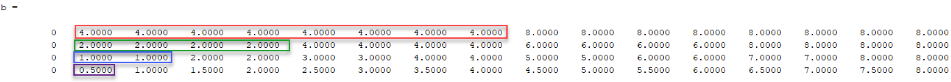
\includegraphics[width=\textwidth]{papers/wavelets/images/17-2_BspFillUp.png}
	\caption{Beispiel für die Matrixbefüllung wie sie im CWT-Code
	umgesetzt wird, am Beispiel einer mit $2^k$ steigenden
	Frequenz $k$.
	Im schwarzen Rahmen sind dabei die betrachteten Frequenzen angeben.
	In der unteren Graphik wird die Befüllung der Matrix anhand
	der Verschiebungswerte $b(a)$ angegeben.
	D.~h.~wenn dieselbe Zahl wie davor in der Spalte steht kam
	es an der Stelle nur zu einer Kopie der Berechnung.
	Nur an den Stellen wo es zu einem Zahlenwechsel kommt, wird
	effektiv das Skalarprodukt mit dem Wavelet der Frequenz $a$
	und dem Signal berechnet.}
	\label{wavelet:fig:BspFillUp}
\end{figure}

Das Wavelet mit 8\,Hz besitzt eine Periode von $1/8$s, wobei der
Verschiebungsfaktor im folgenden Beispiel mit dem Faktor 4 belegt
ist, d.~h.~das Wavelet wird überlappungsfrei verschoben.
Damit ist die minimale Schrittweite bei 8\,Hz gegeben mit $1/8\cdot4=0.5$s.
Mit jeder vorhergehenden Frequenz besitzt das Wavelet bei einer
$2^k$ bezogenen Frequenzänderung eine doppelte zeitliche Ausdehnung.
Dies wird in der Abbildung \ref{wavelet:fig:BspFillUp} mit den
verschieden farbigen Rahmen dargestellt.
Die Spaltenanzahl der $a_n \times b_m$ Matrix ist gegeben über die
höchste Frequenz.
Die Verschiebung $b(a)$ wird an die jeweilige Frequenz angepasst,
wodurch alle unter der maximal untersuchten Frequenz (im Beispiel
bei 8\,Hz) liegenden Frequenzen einen Überschuss an Spalten besitzen.
Solange diese Spalte einer zeitlichen Verschiebung $\leq b(a)$
entspricht, wird diese Zelle bloss mit der ursprünglich errechneten
Information befüllt.
Ein Skalarprodukt zwischen Wavelet und Signal findet immer nur dann
statt, wenn der zeitliche Verschiebungswert der Bezugsspalte $\geq
b(a)$ ist.
Damit kommt es nur an den der Waveletperiode angepassten Verschiebungen
zum Skalarprodukt zwischen Wavelet und Signal.
Ansonsten wird der vorhergehende Spaltenwert übernommen.
Damit kann ein adaptierter Zeitschritt, bezogen auf die Periodenlänge
des Wavelets, bei gegebener Frequenz $a$ erzielt werden, was einer
deutlichen Reduktion von Verrechnungsschritten entspricht.

%Für ein Signal mit einer Zeitdauer von 8s entstehen dadurch folgende Blöcke, für die zeitlichen Ausgaben pro Frequenz. Einfach ausgedrückt: 
%überall da, wo die selbe Zahl steht pro Zeile, wird auch der selbe Wert ausgegeben. Es werden also nur noch Berechnungen an den Stellen gemacht wo es einen Wertewechsel pro Zeile gibt. Was genau der Abbildung %\ref{wavelet:fig:BspFillUp} entspricht.

\subsection{Beispiel einer CWT mit Anlehnung an eine $2^k$ Filterbank analog zur DWT
	\label{wavelets:subsection:Radix2CWT}}
Die wiederholt halbierende Frequenzauflösung kann sowohl am Amplituden-
als auch am Phasengang nachvollzogen werden.
Natürlich ist die Steigerung der Frequenz, um den Faktor zwei pro
Untersuchungsstufe für eine CWT nicht wirklich sinnvoll, weil der
Informationsverlust zwischen den betrachteten Frequenzen schnell
sehr gross wird.
Trotzdem brachte die Methode des Matrixbefüllens, also das Einbringen
eines frequenzangepassten Zeitschrittes, eine 50\% Steigerung der
Rechenzeit bei kleinem Auflösungsverlust.
Dieser Einschub dient deshalb mehr der Visualisierung, einer an die
DWT angelehnten CWT, wenn also die Frequenz pro Untersuchungsstufe
verdoppelt wird.
Damit kann eine Rasterung wie in der schematischen Abbildung
\ref{wavelet:fig:adaptedFrequndTime} erzielt werden.
Ausserdem soll damit eine weitere Visualisierung zur Funktionsweise
der Matrixbefüllung nachgeliefert werden.
Die Abbildung \ref{wavelet:fig:FilterbankAnwendung} zeigt die
Halbierung der Schrittweite $b(a)$ sowohl im Amplituden- also auch
im Phasengang und die damit verbundene Verdoppelung an benötigten
Berechnungen für die $2^k$ höher liegende Frequenz $k$.

In der DWT führt die Verdoppelung der Frequenz zu einer Zunahme der
Detaillierung des Zeitsignals durch die Filterung und ist somit
eine sinnvolle Abstufung.
In der CWT bringt das keinen Mehrwert, da keine Detaillierung,
sondern eine spezifische Frequenz $k$ gesucht ist.
 
\begin{figure}
	\centering
	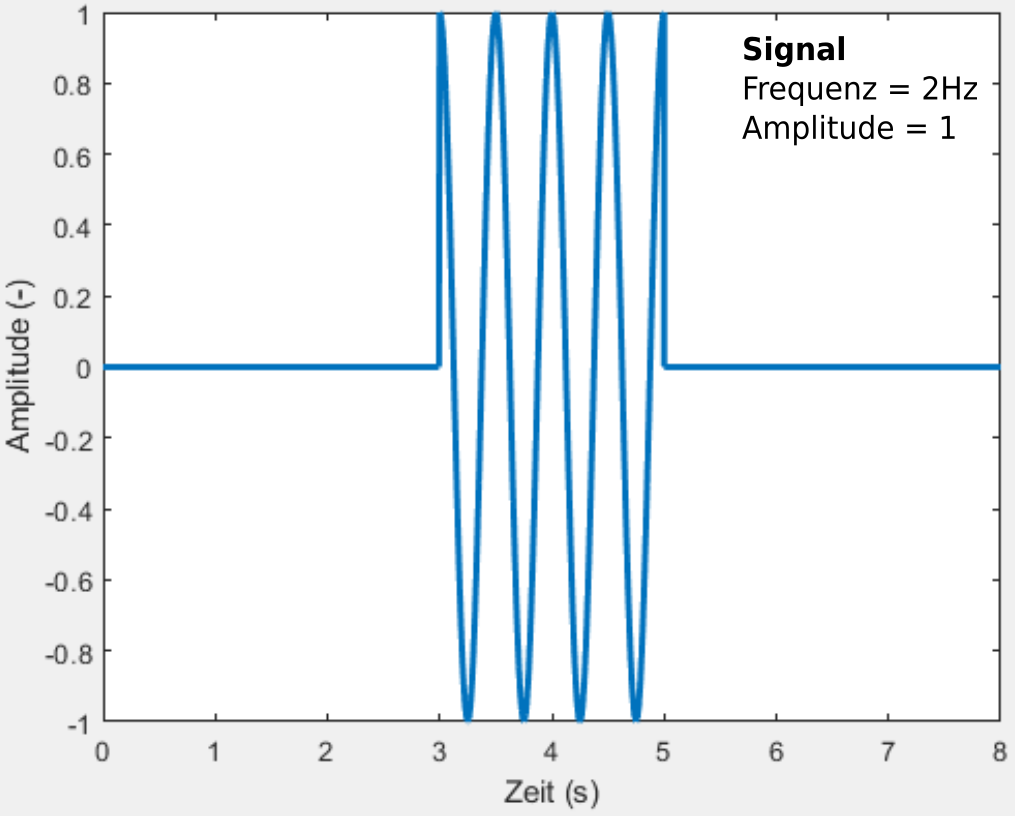
\includegraphics[width=0.5\textwidth]{papers/wavelets/images/17-3_AnwCwtFilterbankSig.png}
	\caption{2\,Hz Beispielsignal zur Untersuchung mit der DWT.
	\label{wavelet:fig:FilterbankAnwendung:beispiel}}
\end{figure}
\begin{figure}
	\centering
	%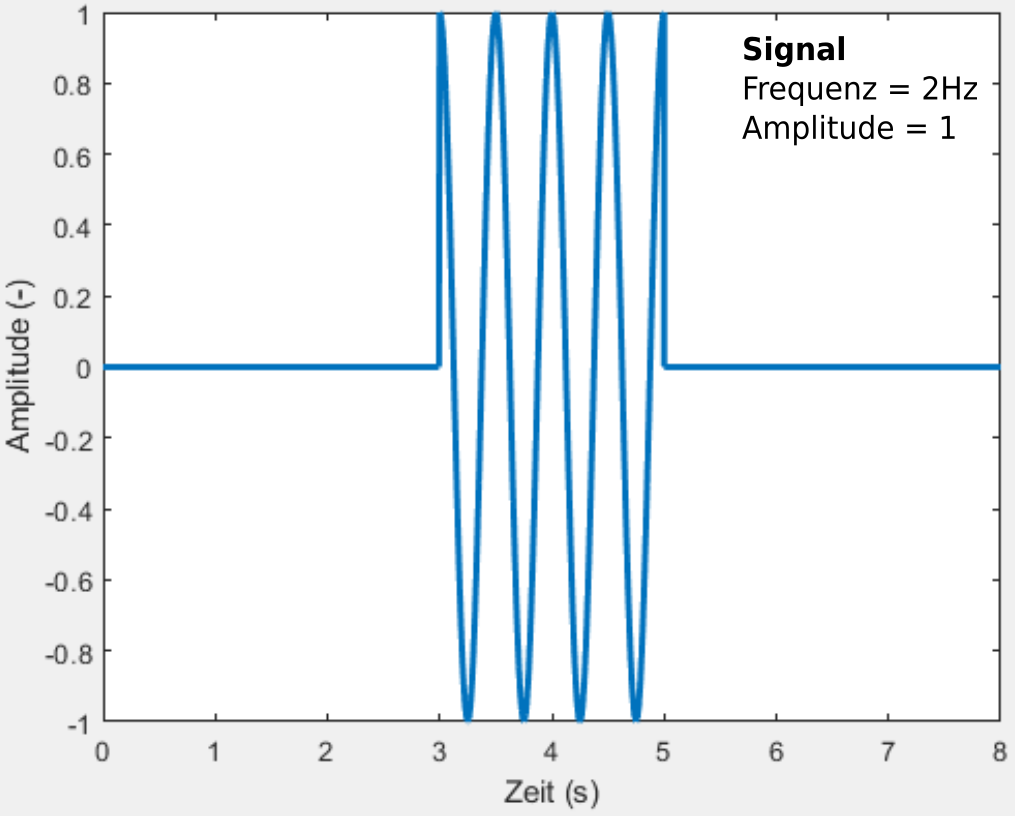
\includegraphics[width=0.3\textwidth]{papers/wavelets/images/17-3_AnwCwtFilterbankSig.png}
	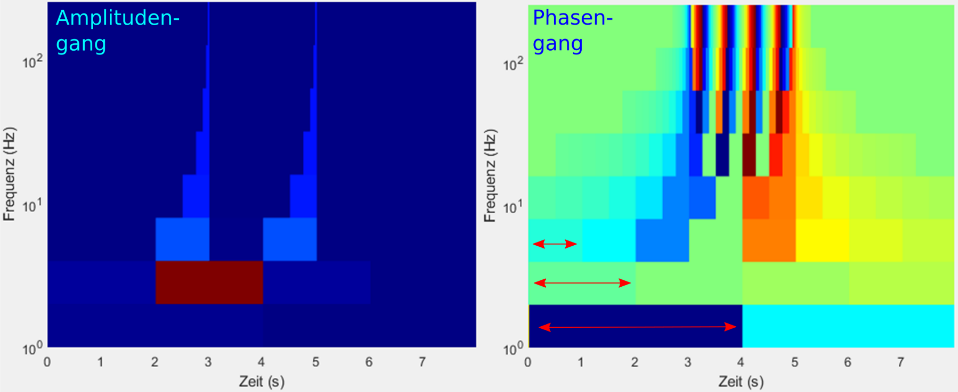
\includegraphics[width=\textwidth]{papers/wavelets/images/17-3_CWT-FilterbankStyle.png}
	\caption{Beispielsignal von
	Abbildung~\ref{wavelet:fig:FilterbankAnwendung:beispiel} untersucht
	mit einer CWT, mit Frequenzabstufung $2^k$, in Anlehnung an die DWT.
	Das Halbieren der Auflösungsstufe ist an Amplituden- und Phasengang
	eindeutig zu erkennen}
	\label{wavelet:fig:FilterbankAnwendung}
\end{figure}

